% % % % % % % % % % % % % % % % % % % % % % % % % % % % % % % % % % % % % % % %
% LaTeX4EI Template for Cheat Sheets                                Version 1.1
%
% Authors: Markus Hofbauer
% Contact: info@latex4ei.de
% Encode: UTF-8
% % % % % % % % % % % % % % % % % % % % % % % % % % % % % % % % % % % % % % % %

% ======================================================================
% Document Settings
% ======================================================================

% possible options: color/nocolor, english/german, threecolumn
% defaults: color, english
\documentclass[english]{latex4ei/latex4ei_sheet}

% set document information
\title{HW/SW Codesign \\ Cheat Sheet}
\author{Fabian Olbert}                    % optional, delete if unchanged
\myemail{fabian.olbert@gmail.com}           % optional, delete if unchanged
% \mywebsite{www.latex4ei.de}          % optional, delete if unchanged
\usepackage{float}
\usepackage{amssymb}

% ======================================================================
% Begin
% ======================================================================
\begin{document}
% Title
% ----------------------------------------------------------------------
\maketitle   % requires ./img/Logo.pdf

% Section
% ----------------------------------------------------------------------
\section{Introduction}

\paragraph{Requirements for HW/SW Systems}
\begin{enumerate}
	\item Reliability
	\item Availability
	\item Serviceability
	\item Safety
	\item Efficiency
	\item Real-time capability
	\item Flexibility
\end{enumerate}

\paragraph{Reliability}

\begin{enumerate}
	\item R(t): Probability that a system works correct until time t presuming it worked correct at a reference time $t_0 = 0$
	\item \textbf{failure rate}: $\lambda$
	\item For constant failure rate $\lambda$: $R(t)= e^{-\lambda t} $
	\item \textbf{Metric}: $MTTF = 1 / \lambda$
	\item \textbf{Reliability of Series Systems}: all n components are functional
	\begin{enumerate}
	\item $R_{sys}(t) = R_1(t) \cdot R_2(t)...R_n(t) = \prod_i^n R_i(t)$
	\item Failure probability: $F(t) = 1 - R(t)$
	\item $R_{sys} \leq min(R_i)$
	\item $\lambda_{sys} = \sum_i^n \lambda_i$ 
	\end{enumerate}
        \item \textbf{Failure of Parallel Systems}: a single path i is functional
	\begin{enumerate}
	  \item $F_{sys}(t) = F_1(t) \cdot F_2(t)...F_n(t) = \prod_i^n F_i(t)$
	  \item $R(t) = 1 - F(t)$
	\end{enumerate}

\end{enumerate}

\paragraph{Availability}
\begin{enumerate}
	\item \textbf{A}: Fraction of time the system works correct in between two consecutive failures
	\item $A = \frac{MTTF}{MTBF} = \frac{MTTF}{MTTF + MTTR}$
	\item Metrics: MTBF (Mean Time Between Failures); MTTR (Mean Time to Repair)
\end{enumerate}

\paragraph{Serviceability}
\begin{enumerate}
	\item Measure considering the time it takes to repair a system after a benign
	\item Metric: MTTR 
\end{enumerate}

\paragraph{Abstraction Levels}

\begin{center}
  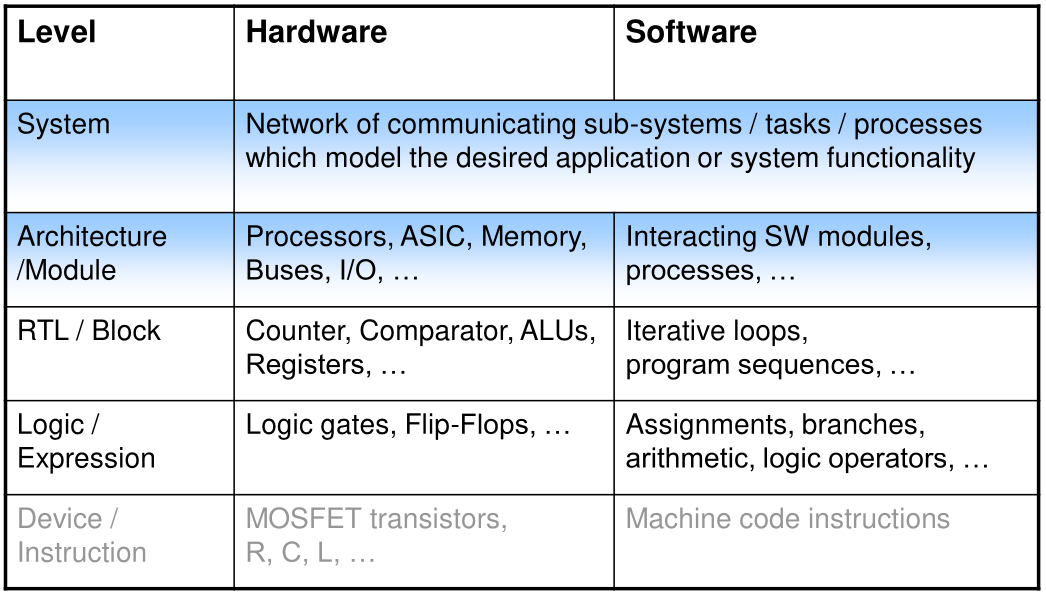
\includegraphics[width=0.8\linewidth]{assets/AbstractionLevels.png}
\end{center}


\section{Methodology}

\textbf{System Design} is the process to implement a desired function with a given set of physical or software components.

\textbf{Design Flow}: Sequence of individual steps of the design process

\textbf{Top-Down Design}
\begin{enumerate}
		\item \textbf{Specification} of the functional behavior
		\item \textbf{Exploration} of alternative realizations within the design space
		\item \textbf{Refinement} of the most promising realization towards the next lower abstraction level
\end{enumerate}

\paragraph{Specification, Exploration, Refinement}

\begin{center}
  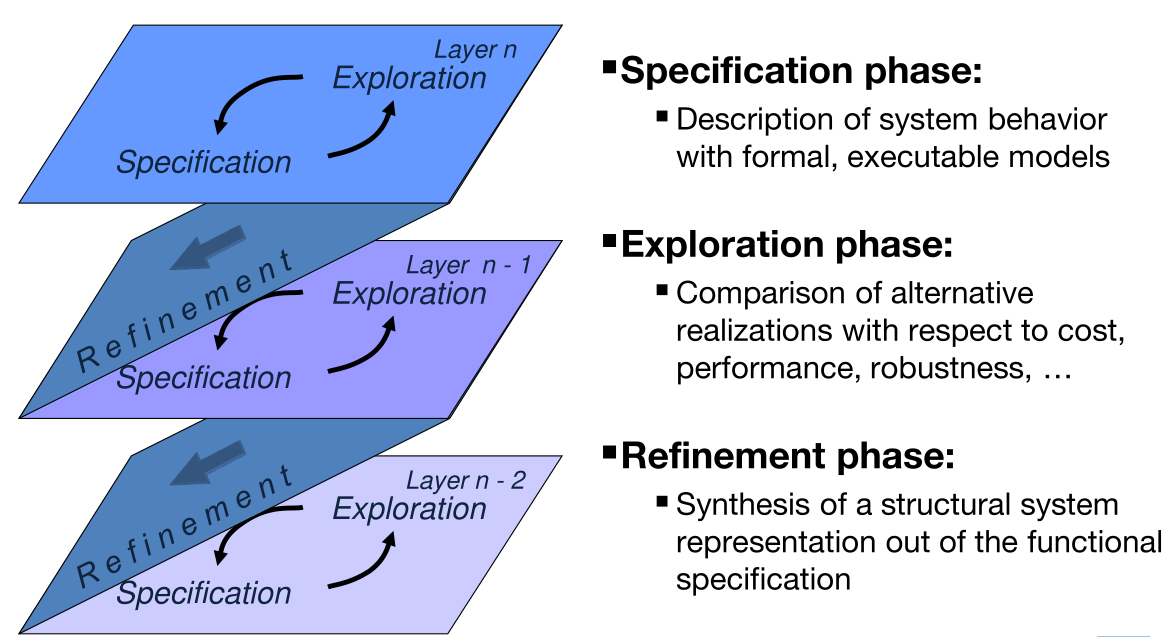
\includegraphics[width=0.8\linewidth]{assets/SpecExRef.png}
\end{center}

\textbf{Abstraction} Design flaws or errors resulting from imprecise modeling or insufficient exploration require abstraction and reiteration of design flow at next higher layer
 
\paragraph{Bottom Up Design}

\begin{center}
  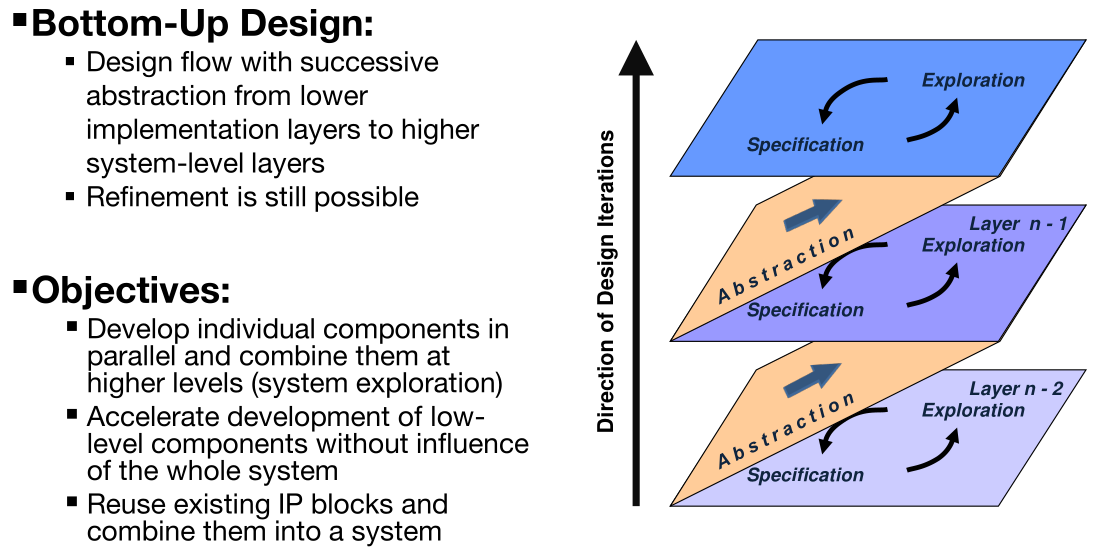
\includegraphics[width=0.8\linewidth]{assets/BottomUpDesign.png}
\end{center}
 
\paragraph{Meet in the Middle Strategy}

\begin{center}
  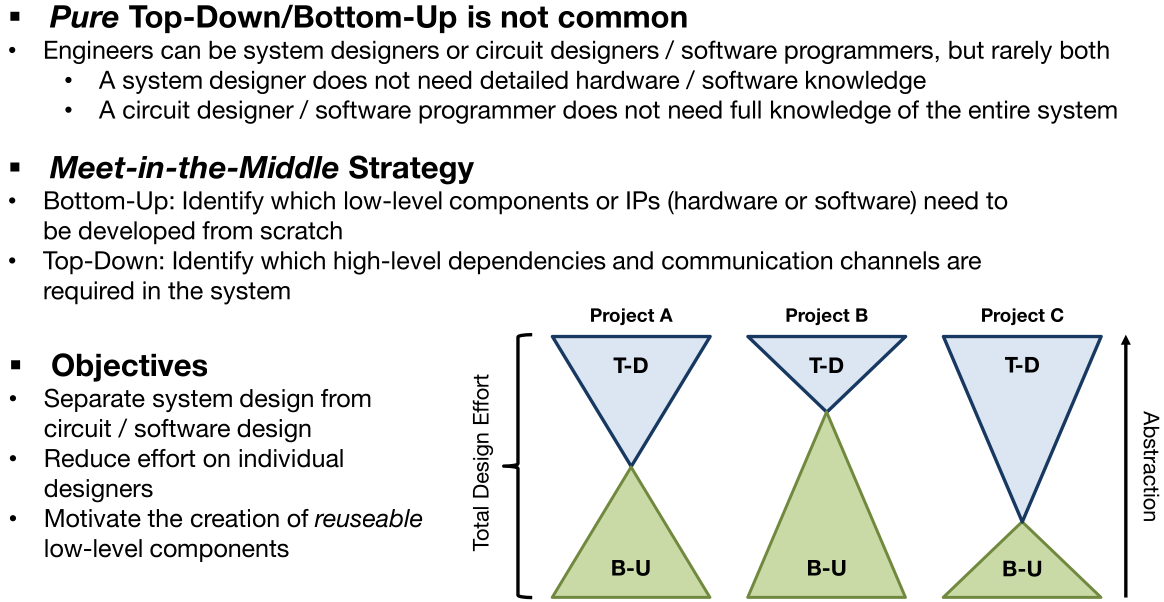
\includegraphics[width=0.8\linewidth]{assets/MeetInTheMiddle.png}
\end{center}

\paragraph{Simulation: Accuracy / Time Effort}

\begin{center}
  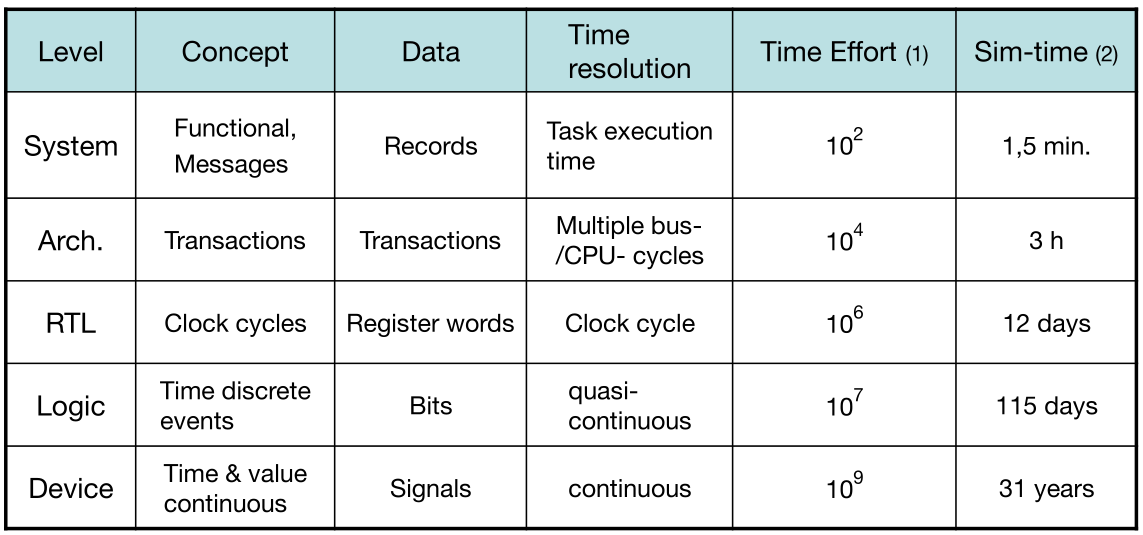
\includegraphics[width=0.8\linewidth]{assets/SimulationAccuracyTime.png}
\end{center}
 
\paragraph{Simualtion Acceleration}
\begin{enumerate}
	\item Divide and Conquer: parallel simulation
	\item Mixed-Level Simulation
\end{enumerate}
 
\paragraph{Design Views}

\begin{center}
  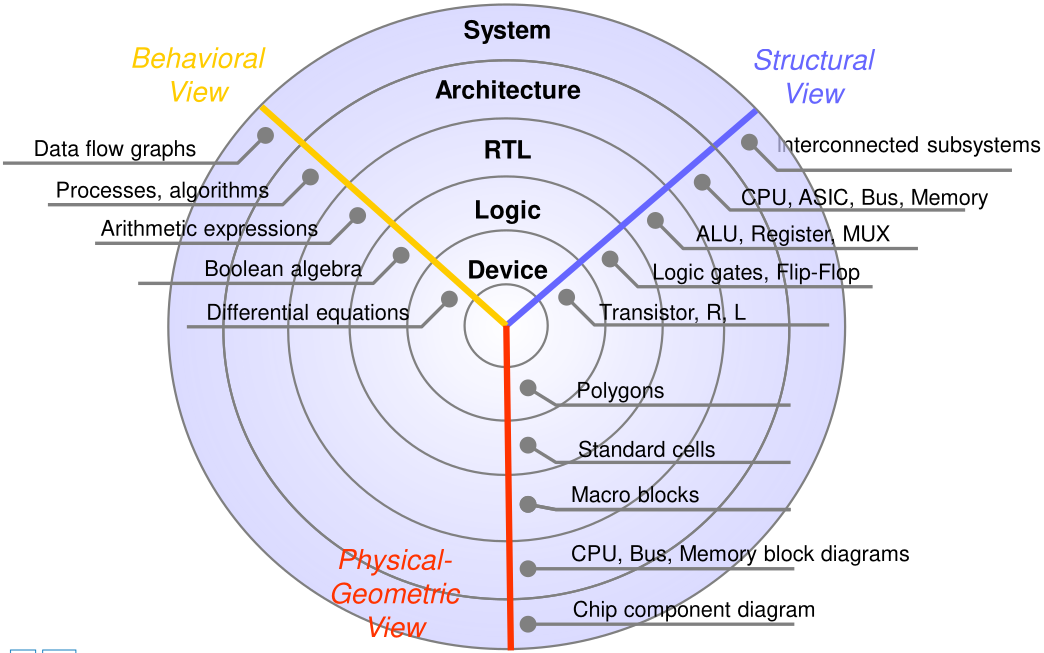
\includegraphics[width=0.8\linewidth]{assets/DesignViews.png}
\end{center}

\paragraph{DesignViewTransition}
\begin{center}
  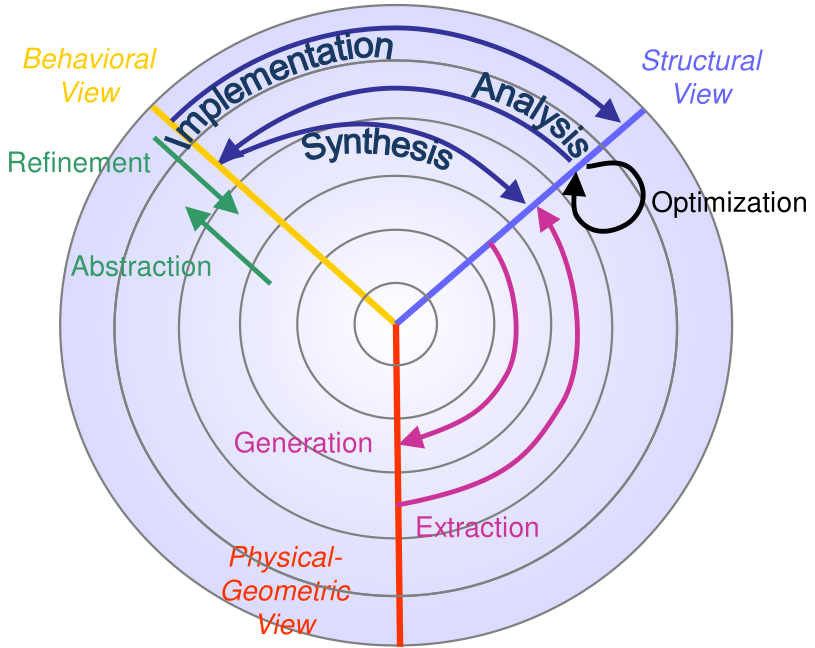
\includegraphics[width=0.7\linewidth]{assets/DesignViewTransitions.png}
\end{center}

\begin{center}
  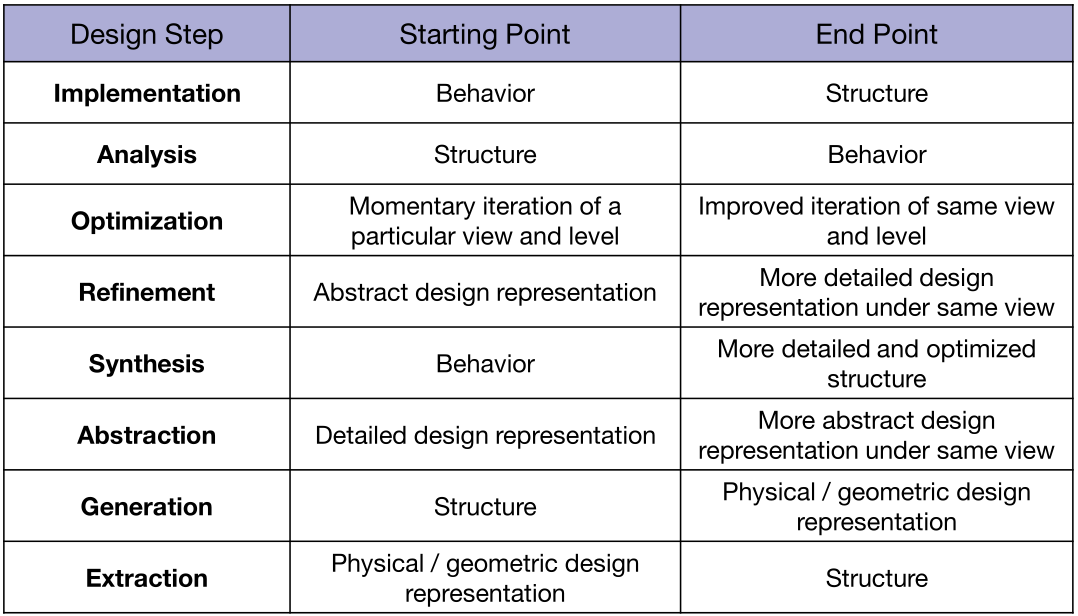
\includegraphics[width=0.8\linewidth]{assets/DesignViewTransitionTable.png}
\end{center}

\begin{center}
  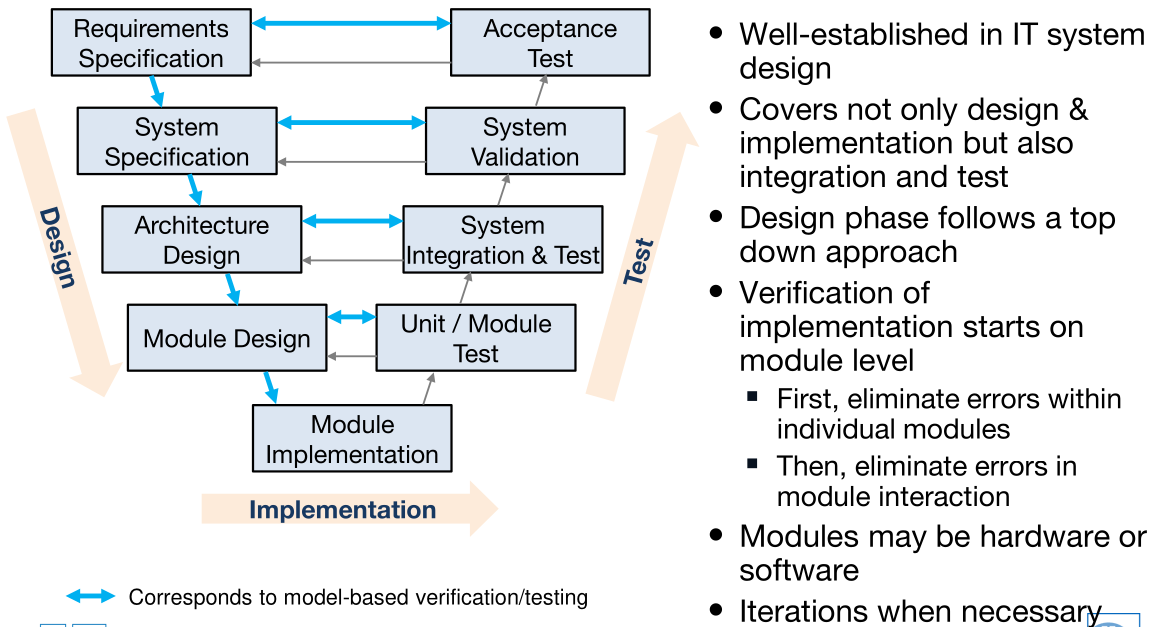
\includegraphics[width=0.8\linewidth]{assets/VModel.png}
\end{center}

\paragraph{Tutorial}

\textbf{linear extrapolation} $\frac{y - y_0}{x - x_0} = \frac{y_1 - y_0}{x_1 - x_0}$

\textbf{finite sum of positive integers} $\sum_{i=1}^{N} = \frac{N(N+1)}{2}$

\textbf{Difference from Solution} $\frac{after - before}{before}$
 
\textbf{Linear Time Complexity} $ O(N)$

\textbf{Quadratic Time Complexity} $ O(N^2)$

\textbf{Linearithmic Time Complexity} $ O(N log_2(N))$

\textbf{Execution Time} $T_{exec} = \frac{CPI \cdot Ops}{f_{cpu}}$
 
\textbf{Optimization} Parallelize tasks that are non dependent, run bottleneck tasks on HW


\section{Specification \& Modeling}

\begin{center}
  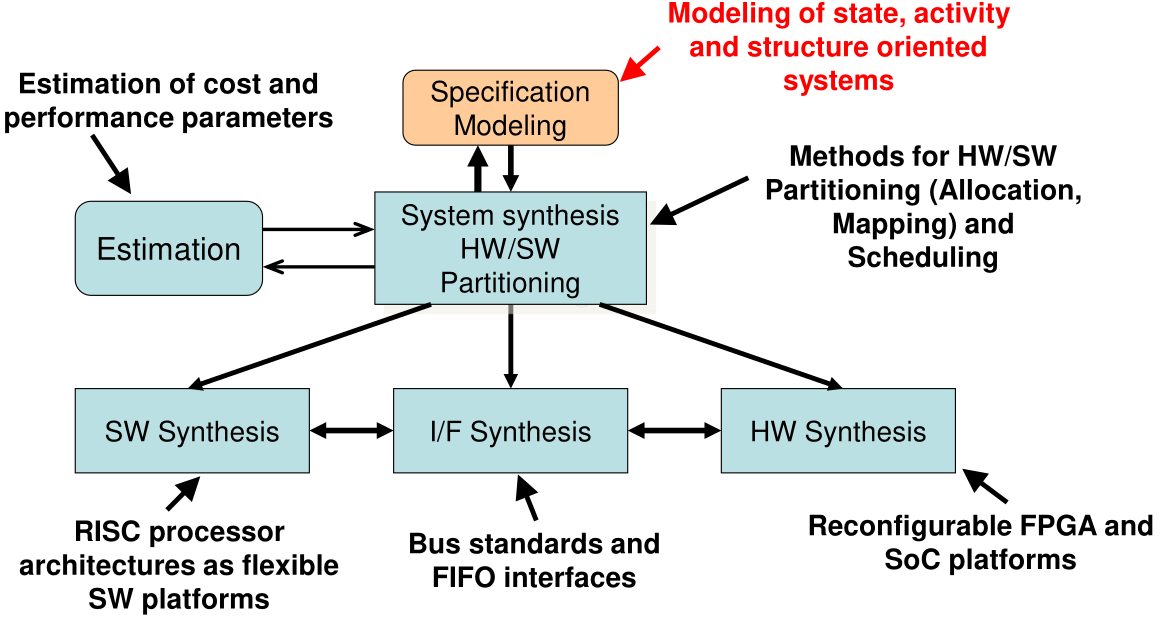
\includegraphics[width=0.8\linewidth]{assets/DesignFlowSystemLevel.png}
\end{center}

\textbf{system specification} defines
\begin{enumerate}
	\item functionality of the system
	\item constrains / properties (latency, power dissipation...)
\end{enumerate}

\textbf{Virtual Prototoypes} Alllow for HW and SW components of a system to be developed in parallel.

\paragraph{Models of Computation}

\begin{center}
  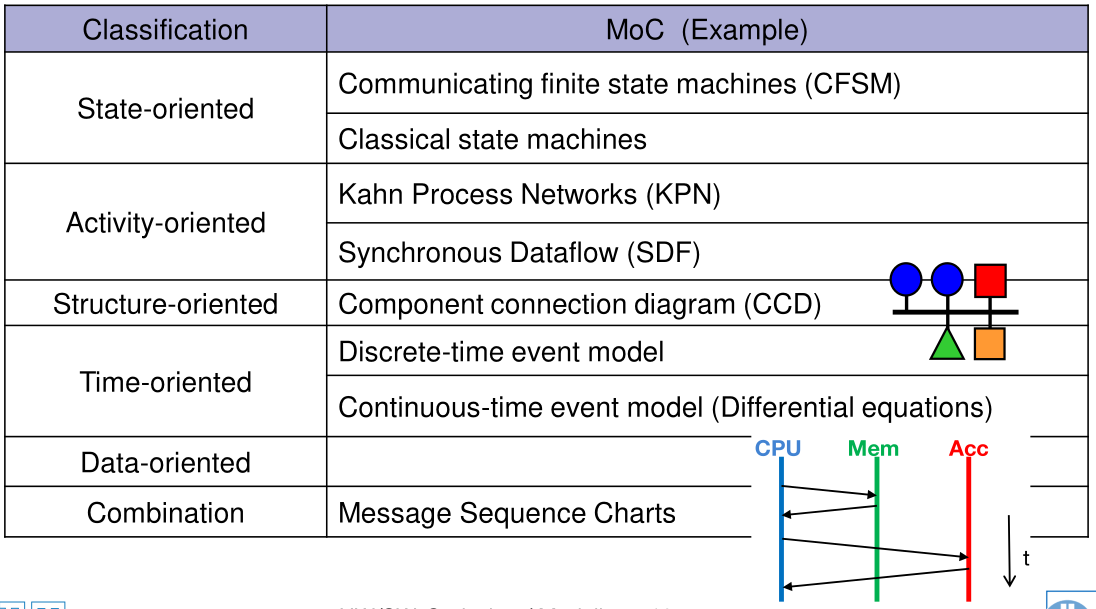
\includegraphics[width=0.8\linewidth]{assets/ModelsOfComputation.png}
\end{center}

\subsection{State-Oriented Models}

\paragraph{Finite State Machine}

\begin{center}[h]
  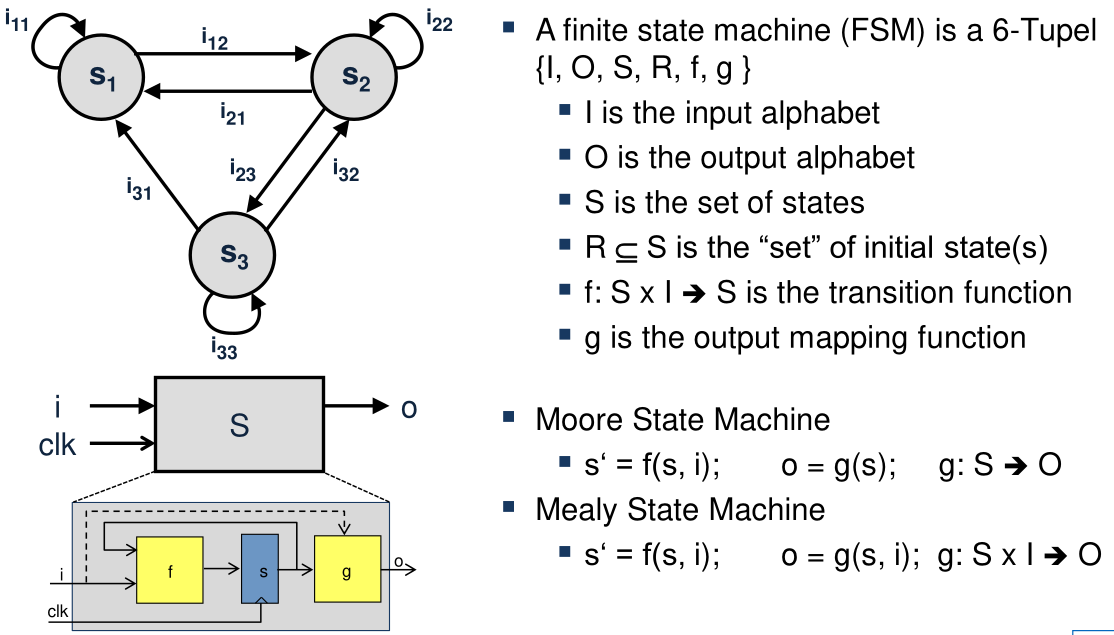
\includegraphics[width=0.8\linewidth]{assets/FiniteStateMachine.png}
  \label{fig:finitestatemachine}
\end{center}

\paragraph{Control Flow Graph}

\begin{center}
  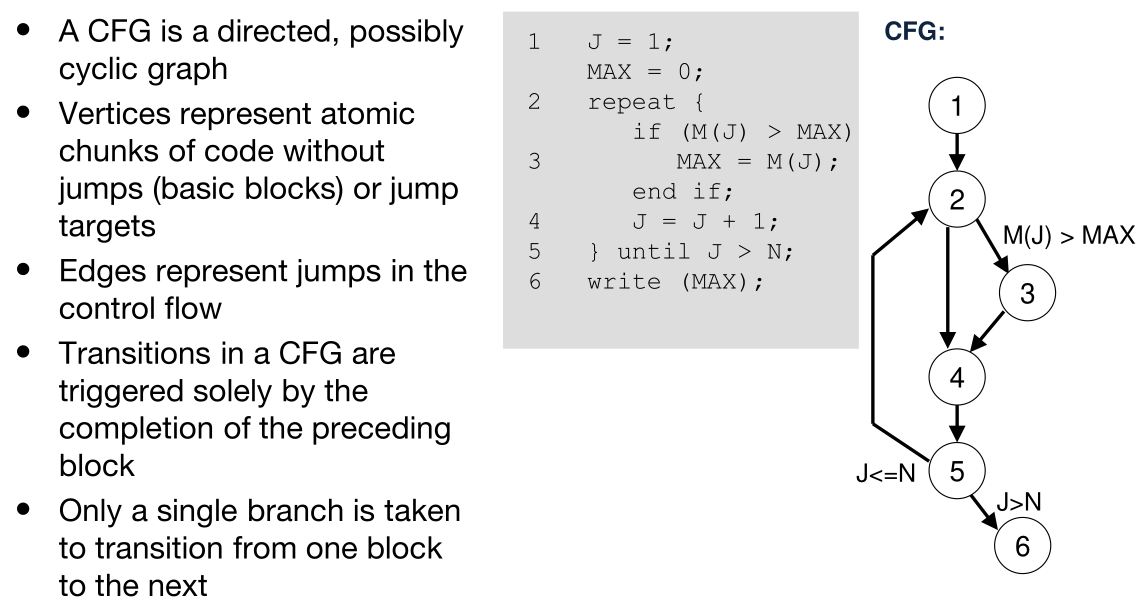
\includegraphics[width=0.8\linewidth]{assets/ControlFlowGraph.png}
  \label{fig:controlflowgraph}
\end{center}

\subsection{Activity Oriented Model}

\paragraph{Data Flow Graph}
 
\begin{center}
  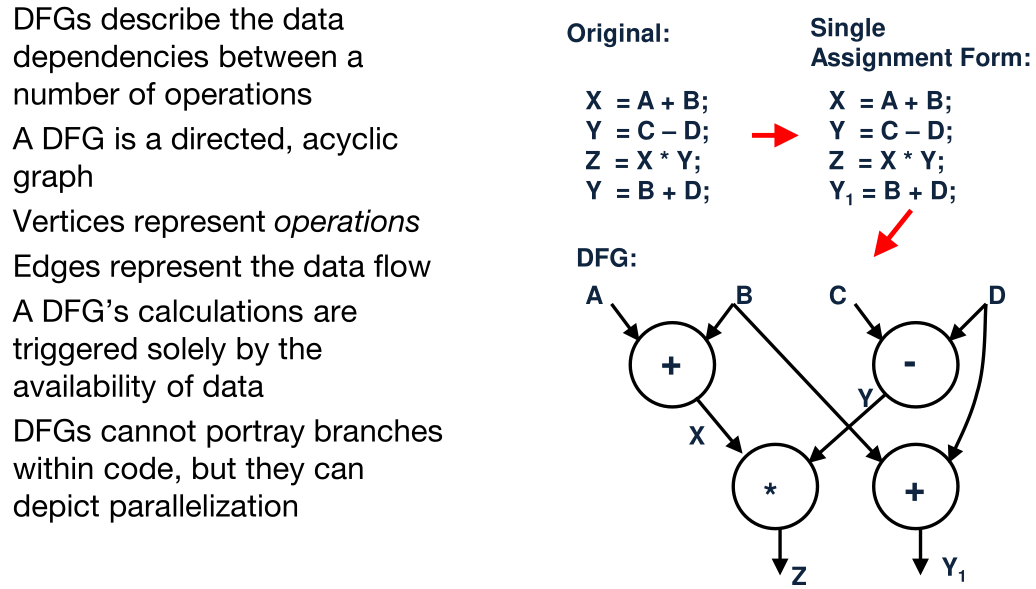
\includegraphics[width=0.8\linewidth]{assets/DataFlowGraph.png}
  \label{fig:dataflowgraph}
\end{center}

\paragraph{Kahn Process Networks (KPNs)}

\textbf{deadlocks}
\begin{enumerate}
  \item \textbf{True deadlock}: read from an empty buffer (KPN read semantics) which is never filled again
\item \textbf{Artificial deadlock}: write into a full buffer (bounded memories) which is never read again
\end{enumerate}

\textbf{Boundness}: Does the schedule require infinite memory?

\textbf{Completeness}: Do all processes get to run indefinitely?

\textbf{Non-Termination}: Will the there be deadlocks?

\textbf{Data driven scheduling}
\begin{enumerate}
	\item execute a process as soon as tokens are available
	\item Does not necessarily find a schedule with bounded buffers even if one exists
	\item Prefers completeness over boundedness
\end{enumerate}

\begin{center}
  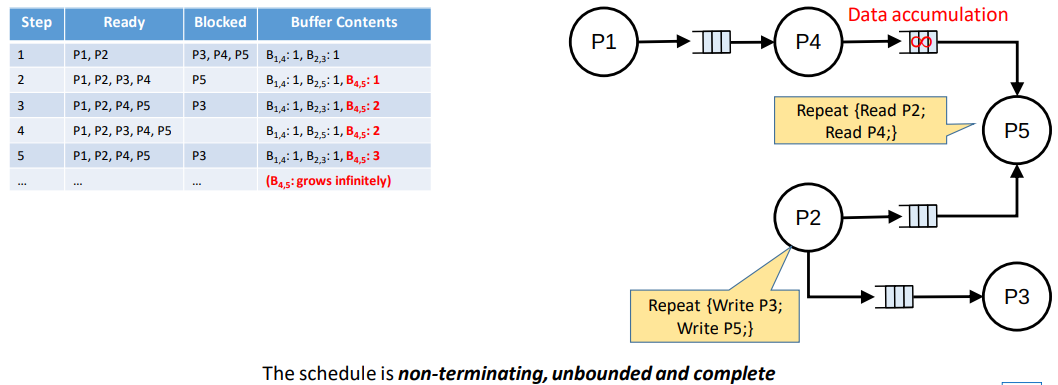
\includegraphics[width=0.8\linewidth]{assets/KPNDataExample.png}
  \label{fig:kpndataexample}
\end{center}

\textbf{Parks' Algorithm}: finds a schedule with bounded buffers if one exists
\begin{enumerate}
	\item Start with buffer size 1 for all channels.
	\item Apply data driven schedule.
	\item If termination occurs, increase buffer sizes by 1.
	\item Repeat.
	\item[$\bullet$] Prefers boundedness over completeness (non-termination)
	\item[$\bullet$] It is not guaranteed that Parks’ Algorithm finds a bounded and complete schedule
\end{enumerate}

\begin{center}
  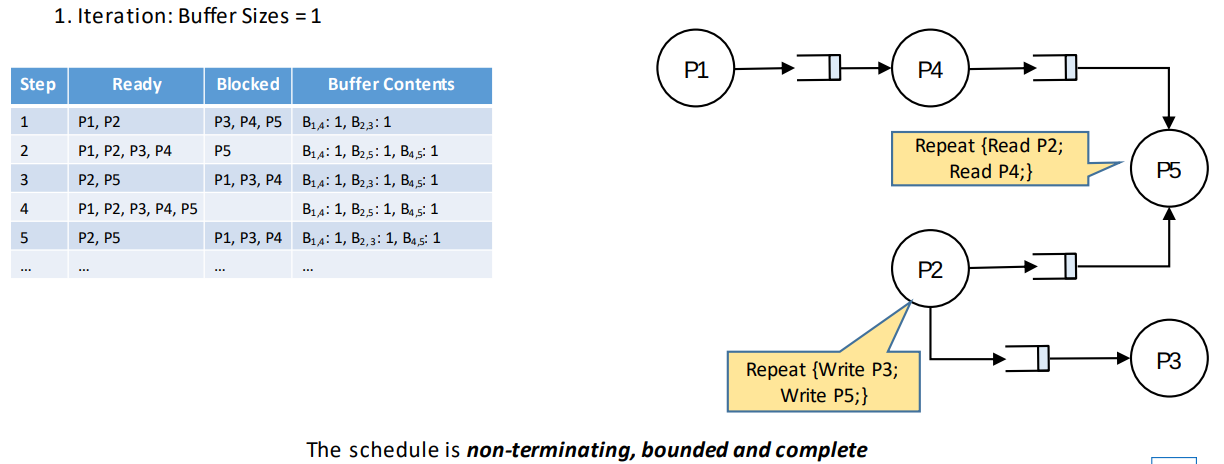
\includegraphics[width=0.8\linewidth]{assets/KPNExamplePark.png}
  \label{fig:kpnexamplepark}
\end{center}
 
\textbf{Properties KPN} No matter what the execution speed or schedule of the processes is, the KPN will always give the same result -$>$ Independent of timing -$>$ deterministic

\subsection{Synchronous Dataflow (SDF)}

\begin{center}
  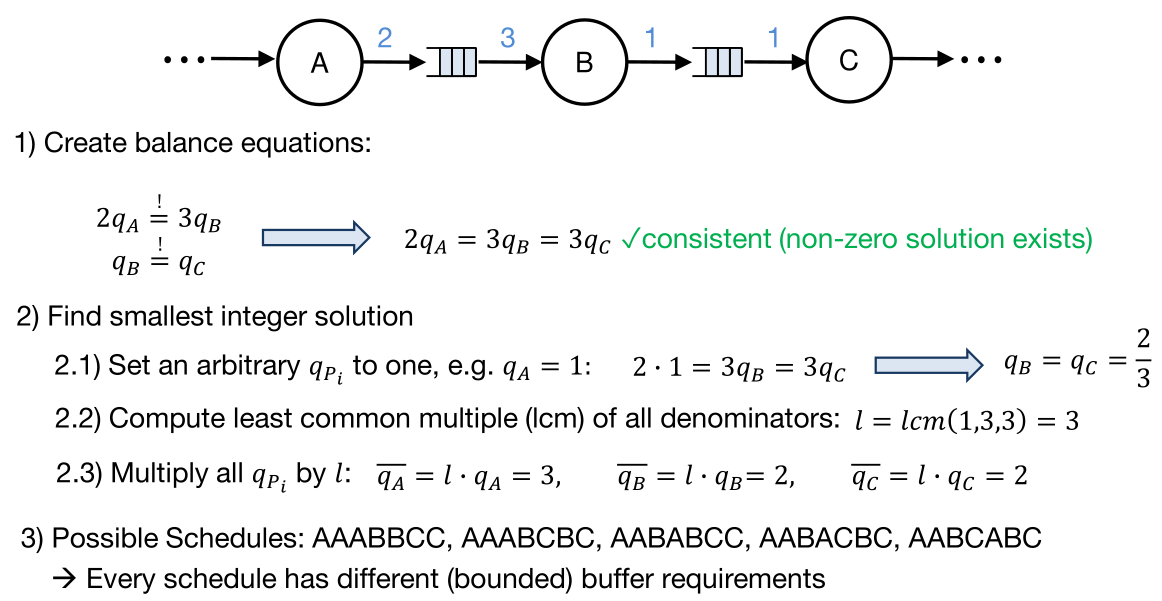
\includegraphics[width=\linewidth]{assets/SDFExample.png}
  \label{fig:sdfexample}
\end{center}
 
\begin{center}
  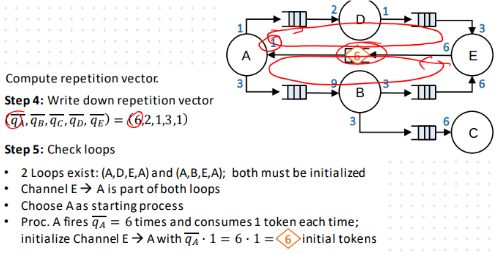
\includegraphics[width=\linewidth]{assets/SDFExample2.png}
  \label{fig:sdfexample2}
\end{center}

\paragraph{Structure Oriented Model}

\paragraph{Data Oriented Model}

\paragraph{Concurrency}

\paragraph{Hierarchy}

\paragraph{Structural-/Behavioral-Hierarchy}

\paragraph{Program Structures/Constructs}

\paragraph{Completion}

\paragraph{Communication}
\begin{enumerate}
  \item Shared-memory communication
    \begin{enumerate}
      \item The sending process writes a global variable into a shared resource (shared memory)
      \item All receiving processes can now read this variable (good broadcasting properties)
      \item Any necessary synchronization must be accomplished separately
    \end{enumerate}
  \item Message passing communication
    \begin{enumerate}
    	\item Data is exchanged between processes using a communication channel to pass messages
	\item Processes can access the channel using send/receive primitives
	\item At higher levels of abstraction, channels are virtual entities and not bound by implementation details
	\item  Channels can be unidirectional or bidirectional, using a point to point or shared (addressed) bus infrastructure
    \end{enumerate}

    \textbf{Blocking transfer} the sending process waits until the receiving process has accepted (or is ready to provide) the data (requires synchronization of the processes prior to the transfer)
    \textbf{non-blocking transfer} the sending process writes the data into a queue and immediately continues processing. The receiving process can then read the data from the queue at its leisure. This allows the sending and receivingprocesses to work independently, but requires additional memory (queues).
\end{enumerate}

\paragraph{Synchronization}
\begin{enumerate}
  \item Control-oriented synchronization
    \begin{enumerate}
    	\item The control structure of the behavioral description determines the synchronization between processes
    \end{enumerate}
  \item Data-oriented synchronization
    \begin{enumerate}
    	\item Synchronization is accomplished using inter-process communication
	  \begin{enumerate}
	    \item Synchronization using shared memory
	    \item Synchronization using message passing
	  \end{enumerate}
    \end{enumerate}
\end{enumerate}
 
\paragraph{Exception Handling} Certain events, such as a reset or CPU interrupt, can necessitate the abrupt termination of a process

\paragraph{Non-Determinism} Occasionally it may be unclear which of several state transitions or
sequences of operations are best suited for the application at hand

\section{Synthesis}

\paragraph{Design Synthesis} 
Combined process of Implementation, Refinement(and Optimization)

\textbf{Central tasks of design synthesis:}

\begin{enumerate}
	\item Allocation: Selection and provisioning of processing resources
	\item Mapping: Assignment of functions to resources
	\item Scheduling: Determination of execution sequences and start times for tasks/processes under consideration of data dependencies in the task graph
\end{enumerate}

\paragraph{System Synthesis}
\begin{enumerate}
  \item Allocation: Determine
    \begin{enumerate}
      \item type and number of CPU/DSP cores,
      \item size of memories,
      \item standard and application specific hardware building blocks,
      \item  I/O interfaces and
      \item interconnect structures
    \end{enumerate}
  \item Mapping: Assignment of entire sub-systems / tasks of the system model to HW / SW resources (HW/SW-Codesign)
    \begin{enumerate}
      \item Scheduling: Determine the
      \item execution sequence of tasks and communication transactions between different resources
      \item execution sequence of tasks which have been mapped to the same resource
    \end{enumerate}
\end{enumerate}

\paragraph{Task Graph}

\begin{center}
  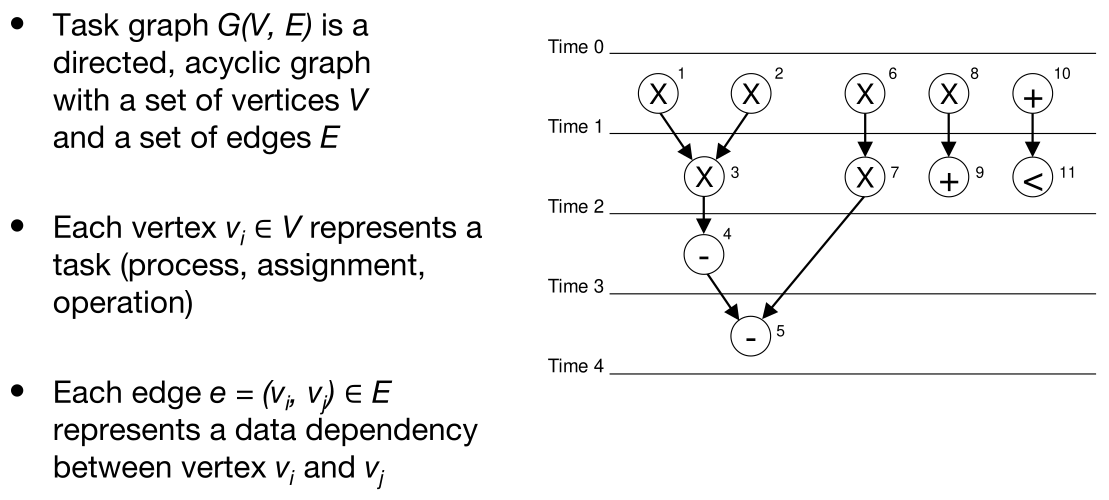
\includegraphics[width=\linewidth]{assets/TaskGraph.png}
  \label{fig:taskgraph}
\end{center}

\paragraph{Resource Graph}

\begin{center}
  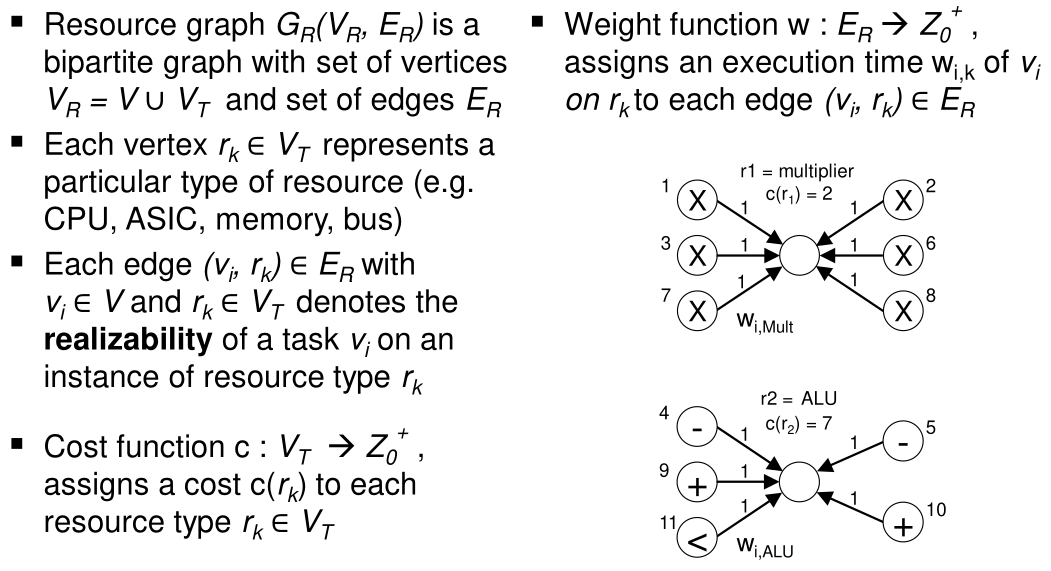
\includegraphics[width=\linewidth]{assets/ResourceGraph.png}
  \label{fig:resourcegraph}
\end{center}

\paragraph{Architecture Graph}

\paragraph{Allocation} Allocation is a function $\alpha$ ..

\paragraph{Mapping}



\section{Scheduling}
\section{Estimation}



% ======================================================================
% End
% ======================================================================
\end{document}
